\documentclass{bachelor_report}

% Додаткові пакети вносіть у цей файл
\input{01_packages}
\addbibresource{../BIB/Resources.bib}

% Додаткові визначення та перевизначення команд вносіть у цей файл
\input{02_redefinitions}

% Відомості про автора роботи
\input{03_data}

% Встановлення числового представлення розділів
\renewcommand{\thesection}{\arabic{section}}

% Встановлення числового представлення підрозділів
\renewcommand{\thesubsection}{\thesection. \arabic{subsection}}

% Налаштування розділів
\titleformat{\section}
{\normalfont\LARGE\bfseries}{\thesection}{1em}{}

% Налаштування підрозділів
\titleformat{\subsection}
{\normalfont\Large\bfseries}{\thesubsection}{1em}{}

% Починаємо верстку документа
\begin{document}

\setfontsize{14}

% Створюємо титульну сторінку
% Титульный лист
\thispagestyle{empty}

\begin{center}
НАЦІОНАЛЬНИЙ ТЕХНІЧНИЙ УНІВЕРСИТЕТ УКРАЇНИ \par
<<КИЇВСЬКИЙ ПОЛІТЕХНІЧНИЙ ІНСТИТУТ ім. Ігоря СІКОРСЬКОГО>>\par
ФІЗИКО-ТЕХНІЧНИЙ ІНСТИТУТ\par

\vspace{40mm}
{\huge Звіт за темою: \par}

\Large\MakeUppercase{\textbf{\reportTitle}} \par
\end{center}

\vspace{40mm}
\begin{flushright}
Виконали: 

студенти групи \reportAuthorGroup

\reportAuthor

\vspace{20mm}
% Науковий керівник:

% \supervisorRegalia

% \supervisorFio

\end{flushright}

\vspace{10mm}
\begin{center}
{Київ~--- 2023}
\end{center}

\newpage


%% Створюємо зміст    % -- розкоментуйте, якщо зміст вам потрібен
%\pagenumbering{gobble}
\tableofcontents
\cleardoublepage
%\pagenumbering{arabic}

\setcounter{page}{2}    %!!! -- продумати, як автоматизувати номер сторінки

%% Якщо ви використовуєте зміст, то прослідкуйте, щоб номер сторінки 
%% співпадав із справжнім!

% Створюємо вступ
%\intro
%!TEX root = ../thesis.tex
% створюємо вступ

% \setcounter{chapter}{1}
% \setcounter{section}{1}
\vspace{-0.5cm}
\section{Мета практикуму}
Ознайомитися з принципами баєсiвського пiдходу в криптоаналiзi, побудувати детермiнiстичну та стохастичну вирiшуючі функцiї для заданих розподілів за допомогою програмної реалiзацiї.

\subsection{Постановка задачі та варіант завдання}
\vspace{-0.5cm}
\hspace{1cm} \textit{Варіант №2}

\vspace{0.5cm}
\begin{tabularx}{\textwidth}{X|X}
	\textbf{Треба виконати} & \textbf{Зроблено} \\
	Опис алгоритмів побудови & \checkmark \\
	Обчислення таблиці ймовірностей $P(\textit{M}|\textit{C})$ & \checkmark \\
	Вивід детерміністичної та стохастичної функцій & \checkmark \\
        Обчислення середніх втрат для вирішуючих функцій & \checkmark \\
\end{tabularx}

% \setcounter{chapter}{2}
% \setcounter{section}{0}

% \section{Результати дослідження}

% Додаємо глави
% Якщо ваша робота містить менше або більше глав - модифікуйте наступні 
% рядки відповідним чином
\section{Хід роботи та опис труднощів}

Для роботи з таблицями та написанням функцій для отримання розподілу шифротекстів, сумісного розподілу відкритих текстів та шифротекстів було обрано використовувати мову C\#.

В результаті було отримано відповідні таблиці ймовірностей, які використовувались безпосередньо для побудови детерміністичної та стохастичної функцій, а також було знайдено значення середніх витрат побудованих функцій.

При виконанні практикуму виникли невеликі труднощі з форматом завантажуваних даних безпосередньо у код, через що було прийнято рішення перезаписати ці дані у вигляді масивів даних для зручності.

%!TEX root = ../thesis.tex

\section{Результати дослідження}
\label{chap:research_results} 

В результаті проробленої роботи було визначено, що детерміністична та стохастична функції вийшли різними, при цьому значення обох середніх похибок у відповідних функціях вийшли однаковими. Таким чином, отримали, що обидві функції досить добре підходять для нашого розподілу.

\subsection{Опис алгоритмів побудови вирішуючих функцій}

Алгоритми побудови вирішуючих функцій схожі між собою і безпосередньо відрізняються лише останнім кроком.

Наведемо алгоритми для обчислення детерміністичної та стохастичної функцій:

\begin{algorithm}
    Побудова детерміністичної вирішуючої функції.
    \begin{itemize}
    \large
        \item Обчислюємо $P(C)$ за формулою:$\forall C: P(C) = \sum_{(M,k):E_k(M)=C} P(M,k)$.
        \item Обчислюємо $P(C)$ за формулою: $\forall (M,C): P(M,C) = \sum_{k:E_k(M)=C} P(M,k)$.
        \item Обчислюємо $P(M|C)$ за формулою $\frac{P(M,C)}{P(C)}$.
        \item З отриманих значень треба обрати максимальні та присвоїти значення $1$ до комірок матриці, де містилось дане максимальне значення. 
    \end{itemize}
\end{algorithm}

\begin{algorithm}
    Побудова стохастичної вирішуючої функції.
    \begin{itemize}
    \large
        \item Обчислюємо $P(C)$ за формулою:$\forall C: P(C) = \sum_{(M,k):E_k(M)=C} P(M,k)$.
        \item Обчислюємо $P(C)$ за формулою: $\forall (M,C): P(M,C) = \sum_{k:E_k(M)=C} P(M,k)$.
        \item Обчислюємо $P(M|C)$ за формулою $\frac{P(M,C)}{P(C)}$.
        \item З отриманих значень треба обрати максимальні та присвоїти значення $\frac{1}{s}$ до тих комірок матриці, де дане максимальне значення повторюється у рядку $s$ разів. 
    \end{itemize}
\end{algorithm}

\newpage
\subsection{Таблиця ймовірностей \textit{P(M|C)}}
\vspace{-1cm}
\begin{figure}[!h]
    \centering
    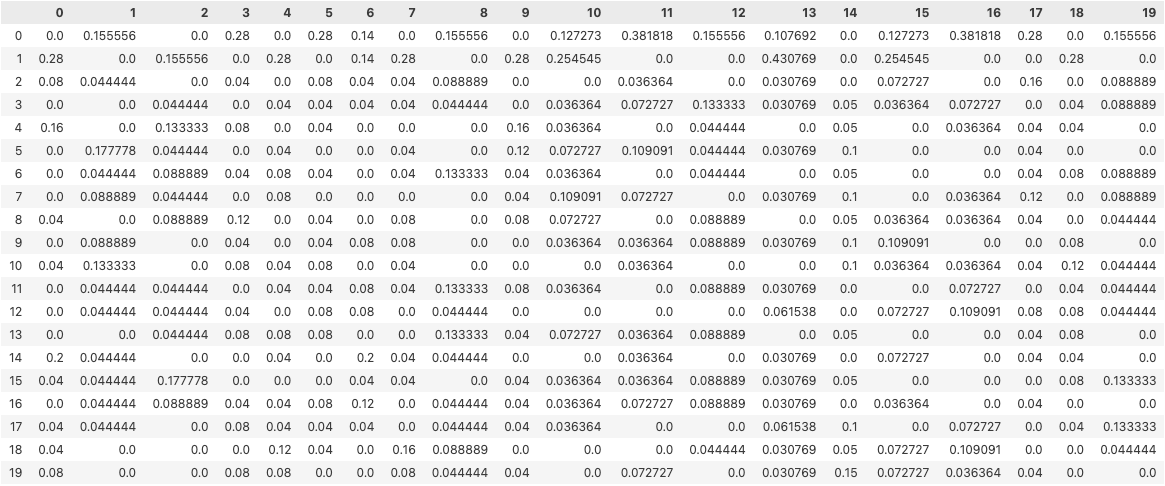
\includegraphics[scale = 0.42]{IMAGES/probabilityTable.png}
    \caption{\large Таблиця умовних ймовірностей для обчислення вирішуючих функцій.}
    \label{fig1}
\end{figure}
\vspace{-0.5cm}
\subsection{Детерміністична та стохастична матриці}
\vspace{-1cm}
\begin{figure}[!h]
    \centering
    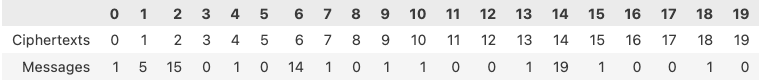
\includegraphics[scale = 0.5]{IMAGES/deterministicMatrix.png}
    \caption{\large Детерміністична вирішуюча ф-я у вигляді відображень (ШТ$\rightarrow$ВТ).}
    \label{fig2}
\end{figure}

\vspace{-1cm}
\begin{figure}[!h]
    \centering
    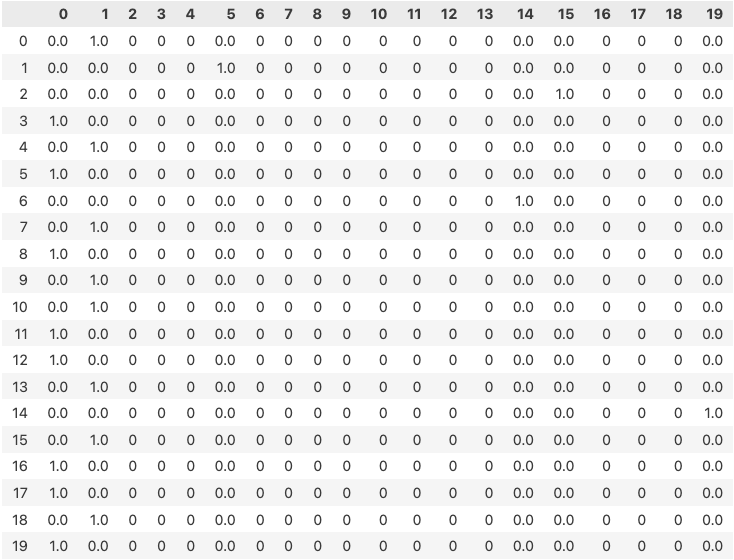
\includegraphics[scale = 0.4]{IMAGES/stohasticMatrix.png}
    \caption{\large Стохастична вирішуюча функція.}
    \label{fig3}
\end{figure}

Також було отримано наступні середні значення втрат:
\begin{itemize}
    \item Для детерміністичної функції: $0.737$
    \item Для стохастичної функції: $0.737$.
\end{itemize}

\section{Висновки}

В даному практикумі за допомогою програмної реалізації практично ознайомилися з баєсівським підходом в криптоаналізі, проаналізували та описали побудову алгоритмів. Також за допомогою програмної реалізації побудували детерміністичну та стохастичну функції для заданих розподілів.

% Створюємо висновки
% \conclusions
% \input{../CHAPTERS/w1_conclusions}

% Нарешті
\end{document}